\chapter{Compressive Sensing Architechtures}\label{sec:sensingmodel}

\subsection{Modulated Wideband Converter}
We consider a radio environment with a single primary user (PU) and a network of \(J\) nodes collaboratively trying to sense and reconstruct the PU signal, either in a fully distributed manner (by local communication), or by transmitting measurements to a fusion centre which then solves the linear system. 

We try to sense and reconstruct a wideband signal, divided into \(L\) channels. We have a (connected) network of \(J\) (= 50) nodes placed uniformly at random within the square \(  \left[0,1\right]\times \left[0,1\right] \). This is the same model, as in \cite{Zhang2011b}. The calculations which follow are taken from \cite{Zhang2011b} as well.

The nodes individually take measurements (as in \cite{mishali2010theory}) by mixing the incoming analogue signal \(x\left(t\right)\) with a mixing function \(p_i\left(t\right)\) aliasing the spectrum. \(x\left(t\right)\) is assumed to be bandlimited and composed of up to \(k\) uncorrelated transmissions over the \(L\) possible narrowband channels - i.e. the signal is \(k\)-sparse. 

\begin{figure}[h]
\centering
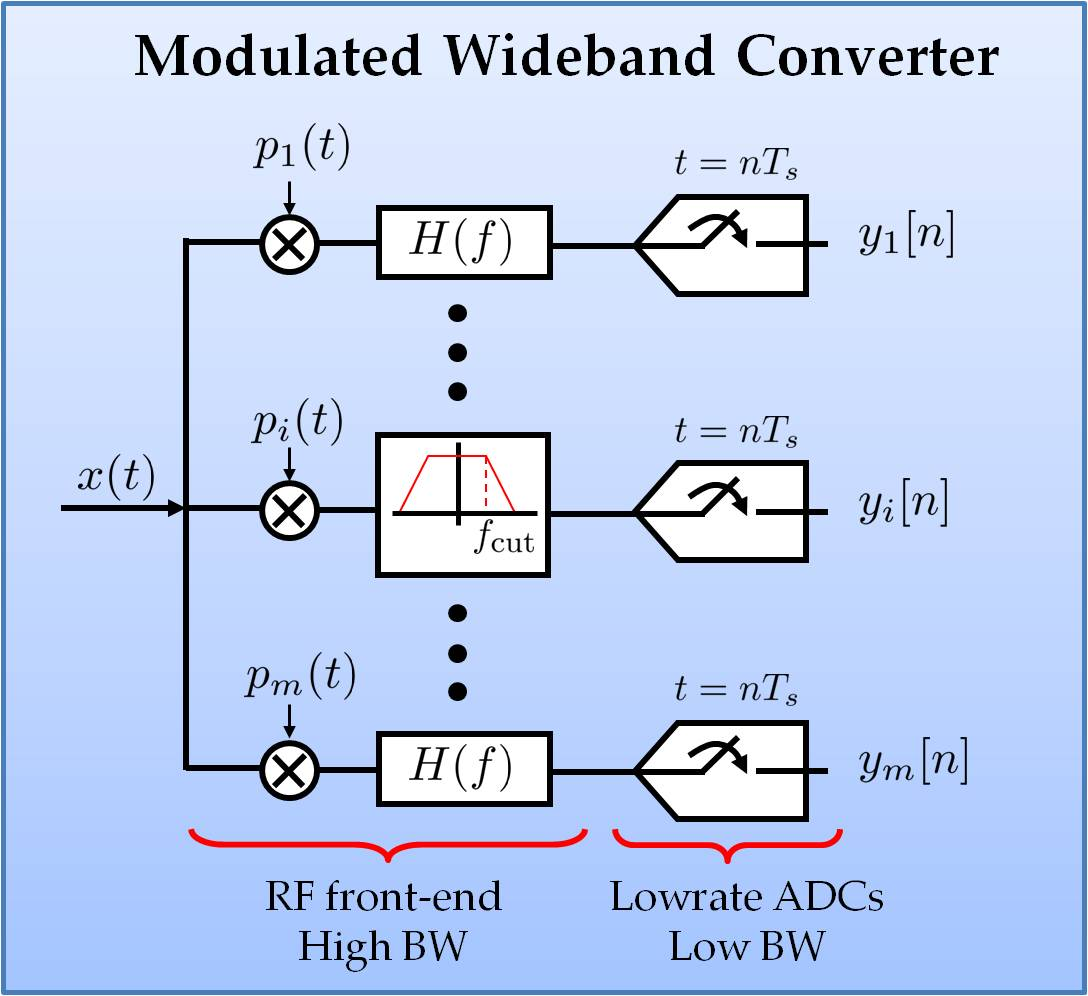
\includegraphics[height = 7.3 cm]{Modulated_wideband_converter.jpg}
\caption{Mse vs SNR for the sensing model, with AWGN only, showing the performance of distributed and centralised solvers}
\label{msevssnr0}
\end{figure}

The mixing functions - which are independent for each node - are required to be periodic, with period \(T_p\). Since \(p_i\) is periodic it has Fourier expansion:

\begin{equation}
p_i\left(t\right) = \sum_{l=-\infty}^{\infty} c_{il} \exp\left({jlt\frac{2\pi}{T_p}}\right)
\end{equation}

The \(c_{il}\) are the Fourier coefficients of the expansion and are defined in the standard manner. The result of the mixing procedure in channel \(i\) is therefore the product \(xp_i\), with Fourier transform (we denote the Fourier Transform of \(x\) by \(X\left( \dot{.} \right)\)):

\begin{align}
X_{i}\left(f\right) &=& \int_{-\infty}^{\infty} x\left(t\right) p_i\left(t\right) dt \nonumber
\\ &=& \sum_{l=-\infty}^{\infty} c_{il} X\left(f-lf_p\right)
\end{align}

(We insert the Fourier series for \(p_i\), then exchange the sum and integral). The output of this mixing process then, is a linear combination of shifted copies of \(X\left(f\right)\), with at most \(\lceil f_NYQ/f_p\rceil\) terms since \(X\left(f\right)\) is zero outside its support (we have assumed this Nyquist frequency exists, even though we never sample at that rate).

This process is repeated in parallel at each node so that each band in \(x\) appears in baseband.

Once the mixing process has been completed the signal in each channel is low-pass filtered and sampled at a rate \(f_s \geq f_p\). In the frequency domain this is a ideal rectangle function, so the output of a single channel is:

\begin{equation}
Y_i\left(e^{j 2 \pi f T_s }\right) = \sum_{l = -L_0}^{+L_0} c_{il} X\left(f-lf_p\right)
\end{equation}

since frequencies outside of \([-f_s/2, f_s/2]\) will filtered out. \(L_0\) is the smallest integer number of non-zero contributions in \(X\left(f\right)\) over \([-f_s/2, f_s/2]\) - at most \(\lceil f_NYQ/f_p\rceil\) if we choose \(f_s = f_p\). These relations can be written in matrix form as:

\begin{equation}
\textbf{y} = \textbf{A}\textbf{x} + \vec{w}
\label{system}
\end{equation}

where \(\textbf{y}\) contains the output of the measurement process, and \(\textbf{A}\) is a product matrix of the mixing functions, their Fourier coefficients, a partial Fourier Matrix, and a matrix of channel coefficients. \(\textbf{x}\) is the vector of unknown samples of \(x\left(t\right)\). 

i.e. \(\textbf{A}\) can be written: 

\begin{equation}
\textbf{A}^{m\times L} = \textbf{S}^{m\times L} \textbf{F}^{L\times L} \textbf{D}^{L \times L} \textbf{H}^{L \times L}
\end{equation}

The system  \ref{system} can then be solved (in the sense of finding the sparse vector \(\vec{x}\) by convex optimisation via minimising the objective function:

\begin{equation}
\frac{1}{2}\|\textbf{Ax}-\textbf{y}\|_2^2 + \lambda \|\textbf{x}\|_1
\end{equation}

where \(\lambda\) is a parameter chosen to promote sparsity. Larger \(\lambda\) means sparser \(\vec{x}\).

\subsection{Random Demodulator}
We assume that the analogue signal \(x\left(t\right)\) is comprised of a finite number of components from some arbitrary dictionary \(\psi_n\left(t\right)\):

\begin{equation}
x\left(t\right) = \sum_{n=1}^N \alpha_n \psi_n\left(t\right)
\end{equation}

The signal is said to be sparse when there are only a few non-zero \(\alpha_n\). The dictionary elements \(\psi_n\) may have a relatively high bandwidth, but the signal itself will have only a few degrees of freedom.

The signal acquisition method proposed consists of three stages (all analogue processing): demodulation, filtering and uniform sampling. 

Initially, the signal is modulated by a pseudo-random sequence \(p_c\left(t\right)\), which alternates at frequencies at (or above) the Nyquist frequency of \(x\left(t\right)\). The signal is then filtered, through a filter with impulse response \(h\left(t\right)\), before being sampled at rate \(\mathcal{M}\) with a traditional ADC.

The output of this system, \(y\left[m\right]\), can be related to the input \(x\left(t\right)\) via a linear transformation of the coefficient vector \(\alpha_n\). 

To find the transformation \(A\), first consider the output of \(y\left[m\right]\), which is the result of convolution and demodulation followed by sampling at rate \(\mathcal{M}\):

\begin{equation}
y\left[m\right] = \int_{-\infty}^{\infty} x\left(\tau\right)p_c\left(\tau\right)h\left(t - \tau\right)\mid_{t = m\mathcal{M}}d\tau
\end{equation}

and by expanding \(x\left(t\right) = \sum_{n=1}^N \alpha_n \psi_n\left(t\right)\):

\begin{equation}
y\left[m\right] =  \sum_{n=1}^N \alpha_n \int_{-\infty}^{\infty} \psi_n\left(t\right)p_c\left(\tau\right)h\left(m\mathcal{M} - \tau\right)d\tau
\end{equation}

we see that the output can be written as:

\begin{equation}
y = Ax
\end{equation}

with

\begin{equation}
A_{m,n} = \int_{-\infty}^{\infty} \psi_n\left(t\right)p_c\left(\tau\right)h\left(m\mathcal{M} - \tau\right)d\tau
\end{equation}

\section{Joint Space-Frequency Model}
We write the power spectral density (psd) of the \(sth\) transmitter as:

\begin{equation}
\phi_s = \sum_b \beta_{bs} \psi_b\left(f\right)
\label{basis_expansion}
\end{equation}
\\ 

This model expresses in psd of the transmitter in a suitable basis - for example \(\psi_b\left(f\right)\) could be zero everywhere except for the set of frequencies where \(f=b\) i.e. \(\psi\) is a rectangular function with height \(\beta_{bs}\) and support \(f\). Other candidates for \(\psi\) include splines (e.g. raised cosines), and complex exponentials. 

Given this, the psd at the \(rth\) receiver is:

\begin{equation}
\phi_r = \sum_s g_{sr}\phi_s = \sum_s g_{sr} \sum _b \beta_{bs}\psi_b\left(f\right)
\end{equation}

where

\begin{equation}
g_{sr} = \exp\left(-||x_r - x_s||_2^\alpha\right)
\end{equation}

is the channel response between the \(sth\) transmitter and the \(rth\) reciver.

This model can be summarised using Kronecker products as follows:

Let \(\tilde{G} = g_sr^T\), \(e_r, e_b\) be unit vectors i.e. they are \(1\) for the \(i^{th}\) receiver or frequency band respectively.

The received power at a receiver (when only a single transmitter is transmitting) can be written:

\begin{equation}
y_r = \left(	e_r^T \bigotimes I_{n_b}\right) y
\end{equation}

with,

\begin{equation}
y = \left( \tilde{G} \bigotimes I_{n_b} \right) \phi
\end{equation}

Now, we have

\begin{equation}
\phi = e_s \bigotimes \phi_s
\end{equation}

so,

\begin{equation}
y = \left( \tilde{G} \bigotimes I_{n_b} \right) \left(e_s \bigotimes \phi_s \right)
\end{equation}

finally we have,

\begin{equation}
y_r = \left(	e_r^T \bigotimes I_{n_b}\right)\left[\left( \tilde{G} \bigotimes I_{n_b} \right) \left(e_s \bigotimes \phi_s \right)\right]
\end{equation}

\(\beta_{bs} \in \re^{1 \times n_b}\), \(g_{sr} \in \re^{n_r \times n_s}\) and \(\psi_{kb} \in 1 \times n_k n_b\) where \(n_k\) is the number of frequency bands (in this example \(n_k = n_b\).

In the absence of knowledge of the location of the transmitters we introduce a grid of \textit{candidate} locations, to make the above model linear. \(s\) now runs over the set of these candidate locations.

The problem of estimating the coefficients, \(\beta\), from noisy observations \(y = \phi_r + N\left(0,1\right)\) is now one that can be tackled by linear regression/convex optimisation.



\section{Results} \label{sec:results}

The model described in section (\ref{sec:sensingmodel}), equation \eqref{system} was simulated, with a wideband signal of 201 channels and a network of 50 nodes (i.e. the signal will be sampled at a 1/4 of rate predicted by Nyquist theory). The mixing patterns were generated from iid Gaussian sources (i.e the matrix S had each entry drawn from an iid Gaussian source). Monte Carlo simulations were performed at SNR values ranging from 5 to 20, and the expected Mean Squared Error (MSE) of solutions of a centralised solver (spgl1) and a distributed solver (ADMM) were calculated over 10 simulations per SNR value. The results can be seen in fig (\ref{msevssnr1}). 

The MSE was calculated as follows:

\begin{equation}
\frac{\vectornorm{Z^k - Z*}}{\vectornorm{Z*}}
\end{equation}

where \(Z^k\) is the result of the algorithm at iteration \(k\), and \(Z^*\) is the optimal solution.

These results indicate that for both centralised and distributed solvers, adding noise to the system results in a degrading of performance. Interestingly note, that the distributed solver seems to (slightly) outperform the centralised solver at all SNRs. This is counter-intuitive, as it would be expected that centralised solvers knowing \textit{all} the available information would outperform distributed solutions. We conjecture that the updates described in section \eqref{sec:opt-on-graphs}, take into account differences in noise across the network. The distributed averaging steps, which form the new prior for each node, then penalise updates from relatively more noisy observations. This corroborates observations from \cite{bazerque2008}.

This observation is (partially) confirmed in figure (\ref{erroriterations}), which plots the progress of the centralised and distributed solvers (as a function of iterations) towards the optimum solution. The SNR is 0.5 (i.e the signal is twice as strong as the noise). Note that after around 300 iterations, the MSE of the distributed solver is consistently below that of the centralised solver.

\begin{figure}[h]
\centering
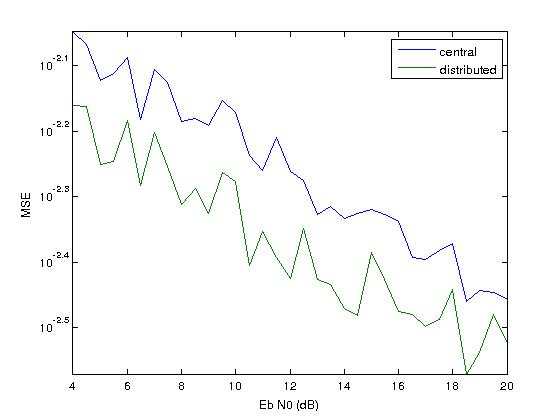
\includegraphics[height = 7.3 cm]{ebn0bbvsmse10ppnoH1logs.jpg}
\caption{Mse vs SNR for the sensing model, with AWGN only, showing the performance of distributed and centralised solvers}
\label{msevssnr0}
\end{figure}

\begin{figure}[h]
\centering
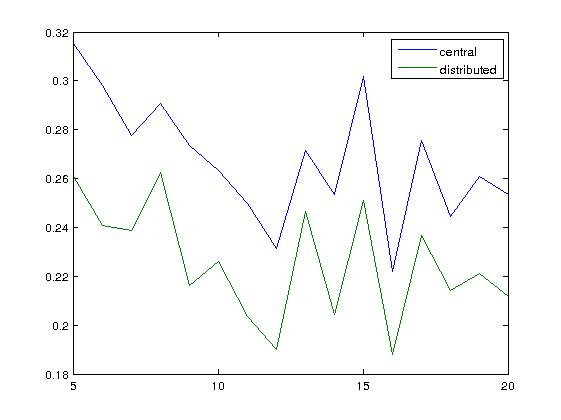
\includegraphics[height = 7.3 cm]{ebn0bbvsmse100ppwithH.jpg}
\caption{Mse vs SNR for the sensing model, showing the performance of distributed and centralised solvers}
\label{msevssnr1}
\end{figure}

\begin{figure}[h]
\centering
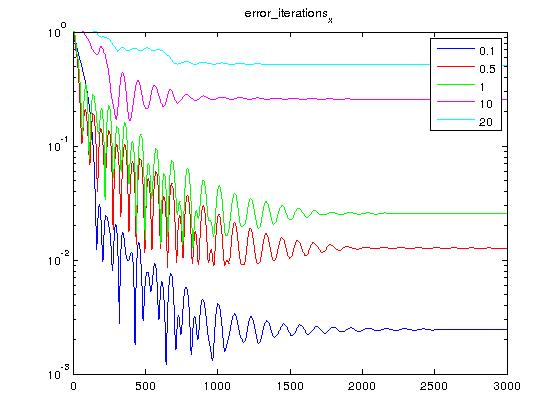
\includegraphics[height = 7.3 cm]{different_lambda.jpg}
\caption{The progress of the distributed solver as a function of the number of iterations, with different values of the regression parameter \(\lambda\)}
\label{fig:differentLambda}
\end{figure}

\begin{figure}[h]
\centering
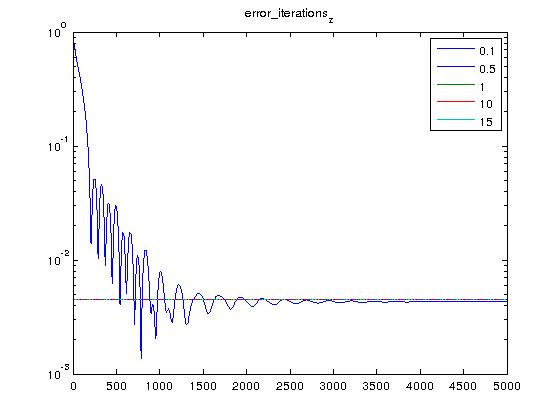
\includegraphics[height = 7.3 cm]{mse_iterations.jpg}
\caption{The progress of a distributed (blue) and a centralised (green) solver as a function of the number of iterations. The value of \(\lambda = 0.1\)}
\label{fig:erroriterations}
\end{figure}

\begin{figure}[h]
\centering
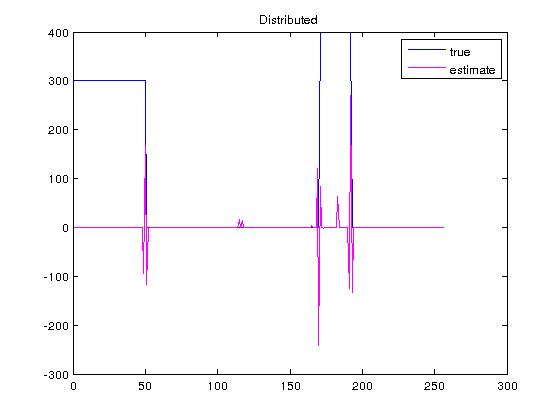
\includegraphics[height = 7.3 cm]{recon_spline.jpg}
\caption{The progress of a distributed (blue) and a centralised (green) solver as a function of the number of iterations. The value of \(\lambda = 0.1\)}
\label{fig:spline_recon}
\end{figure}

\begin{figure}[h]
\centering
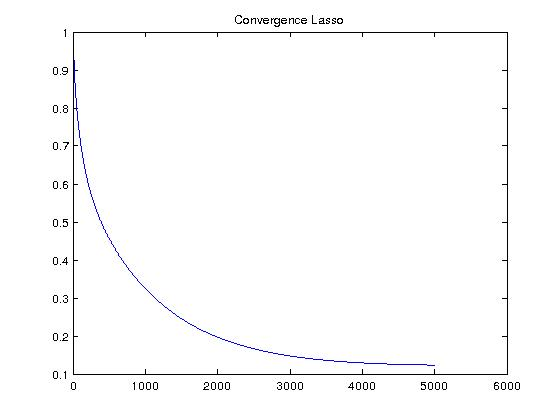
\includegraphics[height = 7.3 cm]{steps.jpg}
\caption{The progress of a distributed (blue) and a centralised (green) solver as a function of the number of iterations. The value of \(\lambda = 0.1\)}
\label{fig:steps_wavelets}
\end{figure}

\begin{figure}[h]
\centering
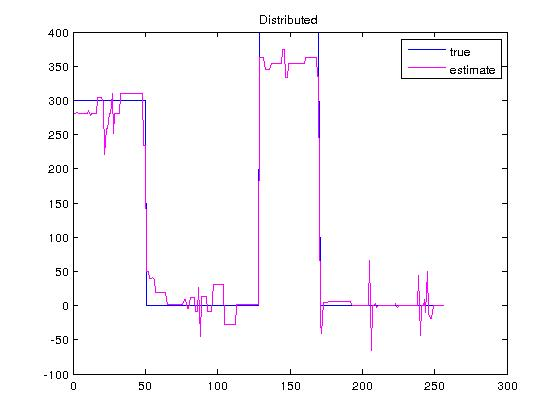
\includegraphics[height = 7.3 cm]{recon170815.jpg}
\caption{The progress of a distributed (blue) and a centralised (green) solver as a function of the number of iterations. The value of \(\lambda = 0.1\)}
\label{fig:wavelet_recon}
\end{figure}

\begin{figure}[h]
\centering
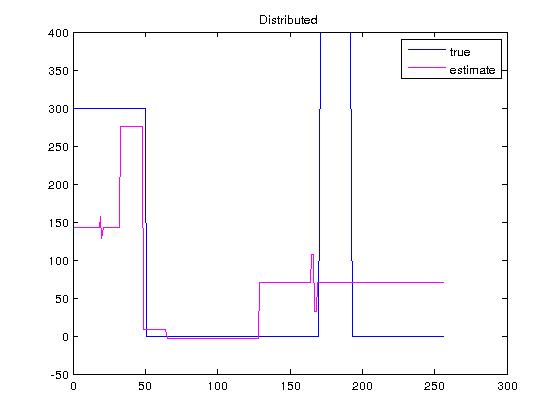
\includegraphics[height = 7.3 cm]{recon_new_bar.jpg}
\caption{The progress of a distributed (blue) and a centralised (green) solver as a function of the number of iterations. The value of \(\lambda = 0.1\)}
\label{fig:wavelet_recon_no_pwer_2}
\end{figure}

\begin{figure}[h]
\centering
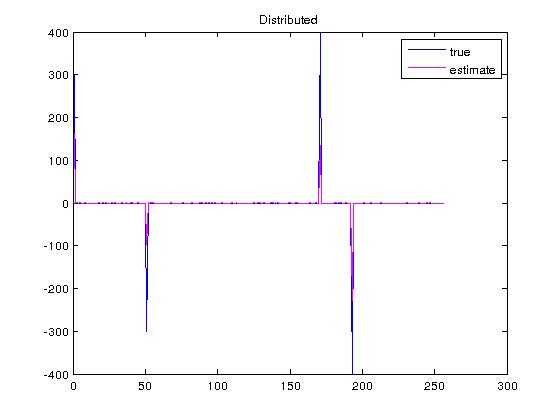
\includegraphics[height = 7.3 cm]{recon_difference.jpg}
\caption{The progress of a distributed (blue) and a centralised (green) solver as a function of the number of iterations. The value of \(\lambda = 0.1\)}
\label{fig:erroriterations}
\end{figure}

\begin{figure}[h]
\centering
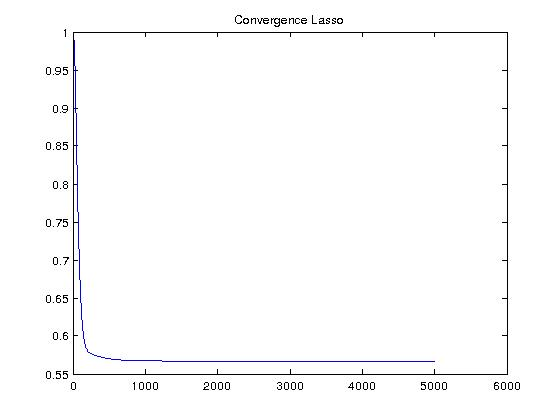
\includegraphics[height = 7.3 cm]{steps_difference.jpg}
\caption{The progress of a distributed (blue) and a centralised (green) solver as a function of the number of iterations. The value of \(\lambda = 0.1\)}
\label{fig:steps_difference}
\end{figure}

\begin{figure}[h]
\centering
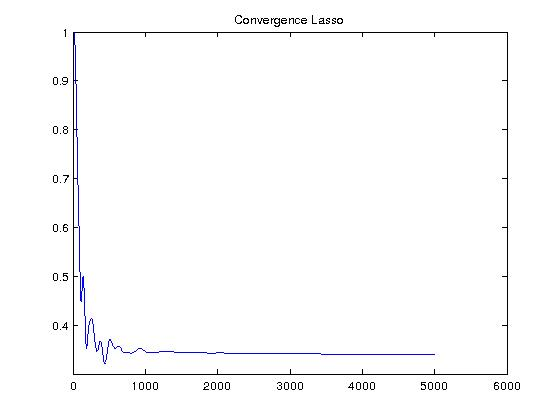
\includegraphics[height = 7.3 cm]{steps_splines.jpg}
\caption{The progress of a distributed (blue) and a centralised (green) solver as a function of the number of iterations. The value of \(\lambda = 0.1\)}
\label{fig:steps_splines}
\end{figure}

\begin{figure}[h]
\centering
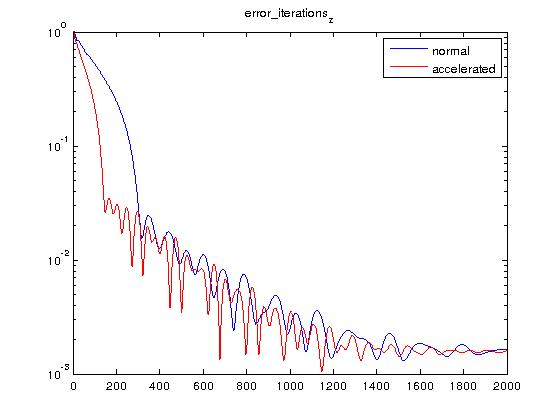
\includegraphics[height = 7.3 cm]{normalvsaccel.jpg}
\caption{The progress of a distributed (blue) and a centralised (green) solver as a function of the number of iterations. The value of \(\lambda = 0.1\)}
\label{fig:steps_splines}
\end{figure}

\section{Conclusions}
We have demonstrated an alternating direction algorithm for distributed optimisation with closed forms for the computation at each step, and discussed the statistical properties of the estimation. 

We have simulated the performance of this distributed algorithm for the distributed estimation of frequency spectra, in the presence of additive (white, Gaussian) and multiplicative (frequency flat) noise. We have shown that the algorithm is robust to a variety of SNRs and converges to the same solution as an equivalent centralised algorithm (in relative mean-squared-error).

We plan to work on larger, more detailed, models for the frequency spectra and to accelerate the convergence via Nesterov type methods to smooth the convergence of the distributed algorithm \cite{goldstein2014fast}. Specifically, we seek to dampen the ringing seen in Figure \ref{fig:erroriterations}
